\begin{center}
  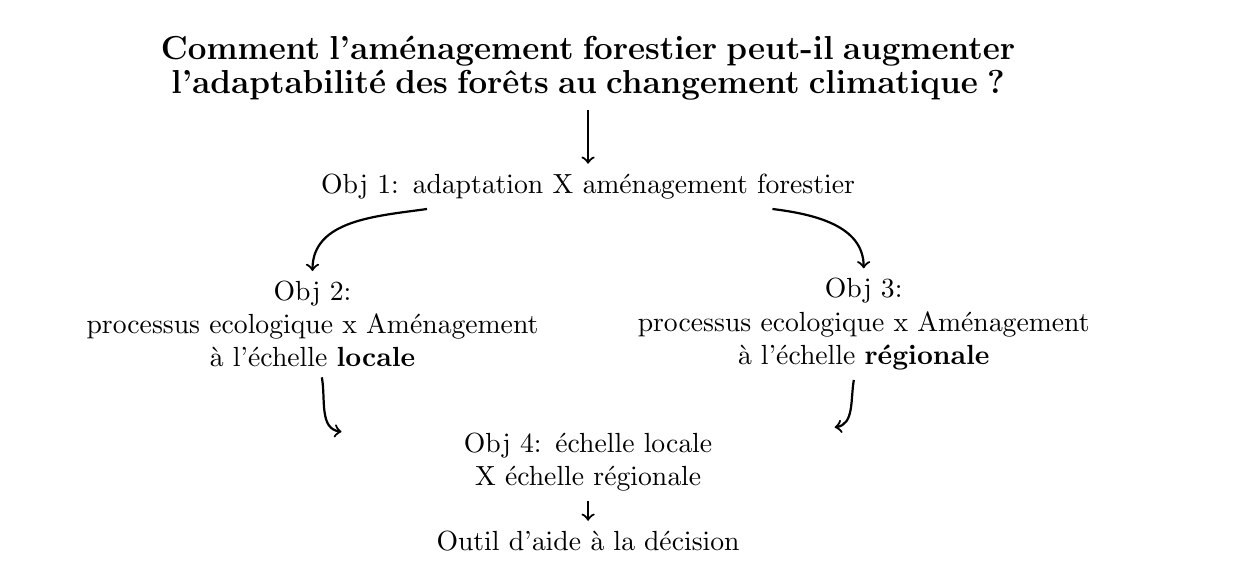
\begin{tikzpicture}[thick,every text node part/.style={align=center}]

    % --------------------------------------------------------- %
    % ------------- principal node (question)
    % --------------------------------------------------------- %
    \node[text width=12cm] (question) at (10,10.25) {\textbf{\large Comment l'aménagement forestier peut-il augmenter \\ \large l'adaptabilité des forêts au changement climatique ?}};

    % --------------------------------------------------------- %
    % ------------ Objectives
    % --------------------------------------------------------- %
    % --- Obj1 node
    \node[text width=10cm] (obj1) at (10,8.75) {Obj 1: adaptation X aménagement forestier};
    \draw [->] (question) edge [out=270, in=90] (obj1);
    % --- Obj2 node
    \node[text width=7cm] (obj2) at (6.5,7) {Obj 2: \\ processus ecologique x Aménagement \\ à l'échelle \textbf{locale}};
    \draw [->] (obj1) edge [out=188, in=90] (obj2);
    % --- Obj2 node
    \node[text width=9cm] (obj3) at (13.5,7) {Obj 3: \\ processus ecologique x Aménagement \\ à l'échelle \textbf{régionale}};
    \draw [->] (obj1) edge [out=353, in=90] (obj3);
    % --- Obj3 node
    \node[text width=6cm] (obj4) at (10,5.25) {Obj 4: échelle locale X échelle régionale};
    \draw [->] (obj2) edge [out=280, in=173] (obj4);
    \draw [->] (obj3) edge [out=260, in=8] (obj4);
    % --- Obj4 node
    \node[text width=6cm] (concl) at (10,4.25) {Outil d'aide à la décision};
    \draw [->] (obj4) edge [out=270, in=90] (concl);

  \end{tikzpicture}
\end{center}
